\section{Introduction}

%motivation
It is well known that a vehicle driving at a constant velocity use less fuel than an accelerating vehicle due to the physical laws of motion.\cite{Vejdir}
%The physical laws of motion say that an accelerating vehicle consumes more fuel than a vehicle driving at a constant velocity.\cite{Vejdir}
In order to save fuel, one should therefore try to drive with a constant speed, but several factors prevents drivers in doing this. 
These factors are for example merging roads, blocking vehicles, traffic incidents and traffic lights. 
It is esimated that 1.8 bilion danish kroner is lost on fuel each year on vehicles stopping for traffic light in Denmark \cite{Vejdir}.

%the problem of traffic lights
Traffic lights hinders the flow of traffic as it blocks vehicles arriving from one direction in order to allow other vehicles to drive through the intersection.
Each direction of the intersection is given a time period in which vehicles are allowed to pass through the intersection. 
Normally, a driver will only be able to guess when the light is going to change based on local knowledge of the area. 

Looking at Figure \ref{fig:Introduction:network} vehicle $\veh_2$ is approacing the intersection.
%If he have spottet a red light for some time, it is likly that the signals are going to change soon. He can either, take the chance and keep driving at the same speed, until the last momment where he need to brake. Or he can slow down and limp toward the intersection and then maybe avoid a full stop at the traffic light. 
Now assume that vehicle $\veh_2$ knows the distance $\dist_3$ where he has to stop for the traffic light. 
Then also assume that vehicle $\veh_2$ knows that in at least $4$ seconds the traffic ligth will change to green. 
Then it is posible to calculate a speed for vehicle $\veh_2$ such that it will drive the distance $\dist_3$ in at least $4$ seconds. 
Now by the time the vehicle reaches the intersection the signal will have changed and a full stop is avoided.
\begin{figure}[htb]
\centering
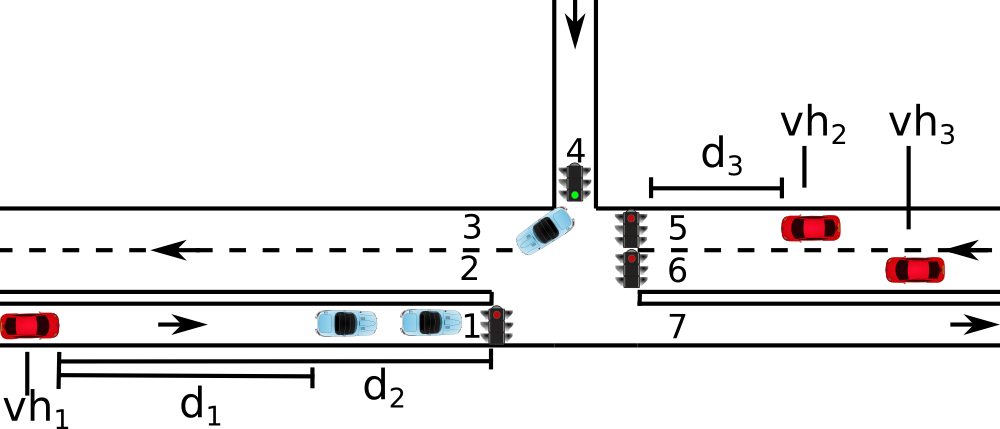
\includegraphics[width=0.5\textwidth]{images/introNetwork.png}
\caption{Eksample network}
\label{fig:Introduction:network}
\end{figure}

Road authorities try to design traffic lights such that the flow of traffic is maximised in all directions.
This can be very difficult, especially in junctions with changing traffic density through out the day.
Two main techniques are used for traffic lights: pretimed traffic controllers, where the signals loop between red, yellow and green in a predefined pattern; and traffic actuated controllers, where approacing vehicles are detected by road-side detectors such that the signals can be adjusted to the current traffic flow. 
The cost of upgrading a traffic light with detectors is 200.000-300.000 danish kroner, not counting extra maintenance costs to repair broken detectors\cite{Vejdir}.

The focus of this article is to investigate whether it is possible to reduce fuel consumption at traffic ligths by matching driving speed to traffic lights. 
We investigate this through simulations with real world map data, traffic data and traffic light programs, both with crossing traffic and road-side senors. %TODO check we do this
We use the traffic simulator SUMO (Simulation of Urban Mobility)\cite{sumo} interfaced via TraCI (Traffic Control Interface)\cite{traci} which is a full scall microscopic traffic simulator.
The system that we propose, is designed with the assumption that very few vehicle will be using it initialy. 
Because of this, we cannot rely on communication between vehicles.
We do, however, assume that traffic lights and vehicles can communicate such that the phases of the traffic lights are avaiable.
We assume the vehicles use a GPS system that handels the communication and that provides a route to travers.
We do not require any further equipment that this.
Additionally, we assume that all drivers follow the rules of traffic, e.g. drives below the speed limit, do not drive into other vehicles and wait for crossing traffic.

%TODO: outline of the article
//Outline of the article


%Modern traffic lights have sensors known as \textit{induction loops} that can detect vehicles driving on the roads.
%These sensors are used to regulate the signals in relation to the number of vehicles approaching the intersection \cite{Vejdir}. %TODO do we need this?
%If it is possible to reduce the stop-and-go behaviour at traffic lights, it might be possible to reduce the fuel consumption.
%section describing terms of traffic traffic light phase, cycle time ect


%model discribing what we do

%section describing problem with sensors \TODO do we need this?
%A traffic light using only a timer to regulate the traffic is relatively easy to predict if the phases and cycle time is known. 
%However, when we introduce induction loops that are are effected by vehicles ariving in an unpredicteble pattern, then the traffic light will also to some extent become unpredicteble. 







